% COMP0197 Applied Deep Learning — Assessed Component 3, Part A
\documentclass[runningheads]{llncs}
\usepackage[T1]{fontenc}
\usepackage{graphicx}
\usepackage{amsmath,amssymb}
\usepackage{booktabs}
\usepackage{subcaption}
\usepackage[hidelinks]{hyperref}

\graphicspath{{../results/figures/}}

\begin{document}

\title{Probabilistic LSTM with Uncertainty Decomposition\\for Remaining Useful Life Prediction}
\titlerunning{Probabilistic LSTM for RUL Prediction}

% TODO: Replace with actual author names
\author{Author A\inst{1} \and Author B\inst{1} \and Author C\inst{1}}
\authorrunning{A. Author et al.}
\institute{Department of Computer Science, University College London, UK\\
\email{\{author.a, author.b, author.c\}@ucl.ac.uk}}

\maketitle

% ============================================================
\begin{abstract}
Accurate Remaining Useful Life (RUL) prediction is critical for condition-based maintenance, yet most deep learning approaches provide only point estimates.
We present a probabilistic LSTM that outputs Gaussian predictive distributions and decomposes uncertainty into aleatoric and epistemic components.
A dual-head architecture trained with Gaussian negative log-likelihood (NLL) captures heteroscedastic data noise, while Monte Carlo (MC) Dropout estimates model uncertainty at inference time.
On the NASA C-MAPSS FD001 benchmark, our model achieves an RMSE of 14.84 ($R^2{=}0.872$), matching the deterministic baseline (RMSE 14.96).
It additionally provides calibrated uncertainty: the 95\% prediction interval achieves 93\% empirical coverage.
Decomposition reveals aleatoric uncertainty dominates (std 12.33 vs.\ epistemic 4.38), indicating data noise as the primary bottleneck.
Sparsification analysis confirms predicted uncertainty correlates with actual error, validating its utility for risk-aware decision-making.

\keywords{Remaining Useful Life \and Uncertainty Quantification \and LSTM \and MC Dropout \and Predictive Maintenance}
\end{abstract}

% ============================================================
\section{Introduction}
\label{sec:intro}

Remaining Useful Life (RUL) prediction estimates cycles until failure, enabling condition-based maintenance in safety-critical domains~\cite{lei2018machinery}.
Deep learning has advanced data-driven RUL prediction substantially: CNNs extract local degradation patterns~\cite{sateesh2016deep,li2018remaining}, LSTMs capture long-range temporal dependencies~\cite{zheng2017long,wu2018remaining}, and Transformers model global attention across time steps~\cite{mo2021multi}.
However, the vast majority of methods output single point estimates.
In practice, maintenance decisions require not only a best estimate of RUL but also a measure of how much that estimate should be trusted.

Predictive uncertainty arises from two sources~\cite{kiureghian2009aleatory}: \emph{aleatoric} uncertainty from irreducible data noise and \emph{epistemic} uncertainty from limited training data.
Distinguishing them is actionable: high epistemic uncertainty signals that more data would help, while high aleatoric uncertainty indicates a fundamental precision limit.
Several UQ methods exist: Bayesian neural networks~\cite{blundell2015weight}, deep ensembles~\cite{lakshminarayanan2017simple}, MC Dropout~\cite{gal2016dropout} (which approximates Bayesian inference with negligible overhead), and heteroscedastic variance heads~\cite{nix1994estimating}.
In the RUL domain, Kraus and Feuerriegel~\cite{kraus2019forecasting} applied MC Dropout to LSTMs, and Biggio et al.~\cite{biggio2021prognostics} combined learned variance with MC Dropout for joint decomposition, though systematic calibration evaluation remains limited.

We present a probabilistic LSTM framework on NASA C-MAPSS FD001 with three contributions:
(1)~a dual-head LSTM predicting Gaussian parameters $(\mu, \sigma)$ for heteroscedastic aleatoric uncertainty;
(2)~MC Dropout ($T{=}100$) for epistemic estimation and full uncertainty decomposition;
(3)~comprehensive UQ evaluation (calibration, PICP, MPIW, sparsification) alongside a deterministic ablation baseline.

% ============================================================
\section{Methods}
\label{sec:methods}

\subsection{Probabilistic LSTM Architecture}
Given a sensor series $\mathbf{X} \in \mathbb{R}^{L \times D}$, we learn $p(y \mid \mathbf{X}) = \mathcal{N}(y;\, \mu(\mathbf{X}),\, \sigma^2(\mathbf{X}))$ with input-dependent mean and variance.
The backbone is a 2-layer LSTM ($H{=}128$, inter-layer dropout $p{=}0.25$).
The final hidden state $\mathbf{h}_L$ passes through dropout and two parallel linear heads:
\begin{align}
    \mu &= \mathbf{w}_\mu^\top \mathbf{h}_L + b_\mu, &
    \sigma &= \exp(\mathbf{w}_\sigma^\top \mathbf{h}_L + b_\sigma) + \epsilon
\end{align}
where $\epsilon{=}10^{-6}$.
The model minimises the Gaussian negative log-likelihood:
\begin{equation}
    \mathcal{L}_{\text{NLL}} = \frac{1}{N} \sum_{i=1}^{N} \left[ \frac{(y_i - \mu_i)^2}{2\,\sigma_i^2} + \frac{\log \sigma_i^2}{2} \right]
\label{eq:nll}
\end{equation}
The $\log\sigma^2$ regulariser prevents trivial variance inflation, enforcing an accuracy--calibration trade-off.

\subsection{MC Dropout for Epistemic Uncertainty}
At test time, dropout remains active across $T{=}100$ forward passes, each yielding $(\mu^{(t)}, \sigma^{(t)})$.
Uncertainty is decomposed as:
\begin{align}
    \hat{\mu} &= \tfrac{1}{T}\textstyle\sum_t \mu^{(t)}, &
    \sigma^2_{\text{ale}} &= \tfrac{1}{T}\textstyle\sum_t (\sigma^{(t)})^2  \label{eq:ale} \\
    \sigma^2_{\text{epi}} &= \tfrac{1}{T}\textstyle\sum_t (\mu^{(t)} {-} \hat{\mu})^2, &
    \sigma^2_{\text{total}} &= \sigma^2_{\text{ale}} + \sigma^2_{\text{epi}}  \label{eq:total}
\end{align}
Aleatoric variance averages the learned noise; epistemic variance measures prediction disagreement across stochastic masks.

\subsection{Baseline and RUL Labelling}
A deterministic LSTM with identical architecture but a single MSE-trained output head serves as ablation baseline.
RUL labels follow piece-wise linear clipping~\cite{heimes2008recurrent}: $y_i = \min(c_{\max} - c_i,\; R_{\text{early}})$ with $R_{\text{early}}{=}125$.

% ============================================================
\section{Experiments}
\label{sec:experiments}

\paragraph{Dataset.}
NASA C-MAPSS FD001~\cite{saxena2008damage} provides 100 run-to-failure and 100 truncated test trajectories of turbofan engines under one operating condition and one fault mode.
Each timestep records 21 sensors and 3 operational settings.

\paragraph{Preprocessing and feature selection.}
Feature selection uses a two-stage data-driven process (Fig.~\ref{fig:eda}).
A variance filter removes 10 near-constant features (std $< 0.01$); a Spearman correlation filter then confirms all 14 remaining sensors have $|\rho|{>}0.1$ with RUL, the strongest being s11 ($\rho{=}{-}0.72$), s4 ($-$0.70), and s12 ($+$0.70).
Features are normalised to $[0,1]$ via MinMaxScaler fit on training data.
Sliding windows of length $L{=}30$ are extracted per engine; the label is the RUL at the final timestep.
Training engines are split 80/20 by engine ID; test sequences use the last 30 timesteps (zero-padded if shorter).

\begin{figure}[t]
\centering
\begin{subfigure}[t]{0.48\textwidth}
    \centering
    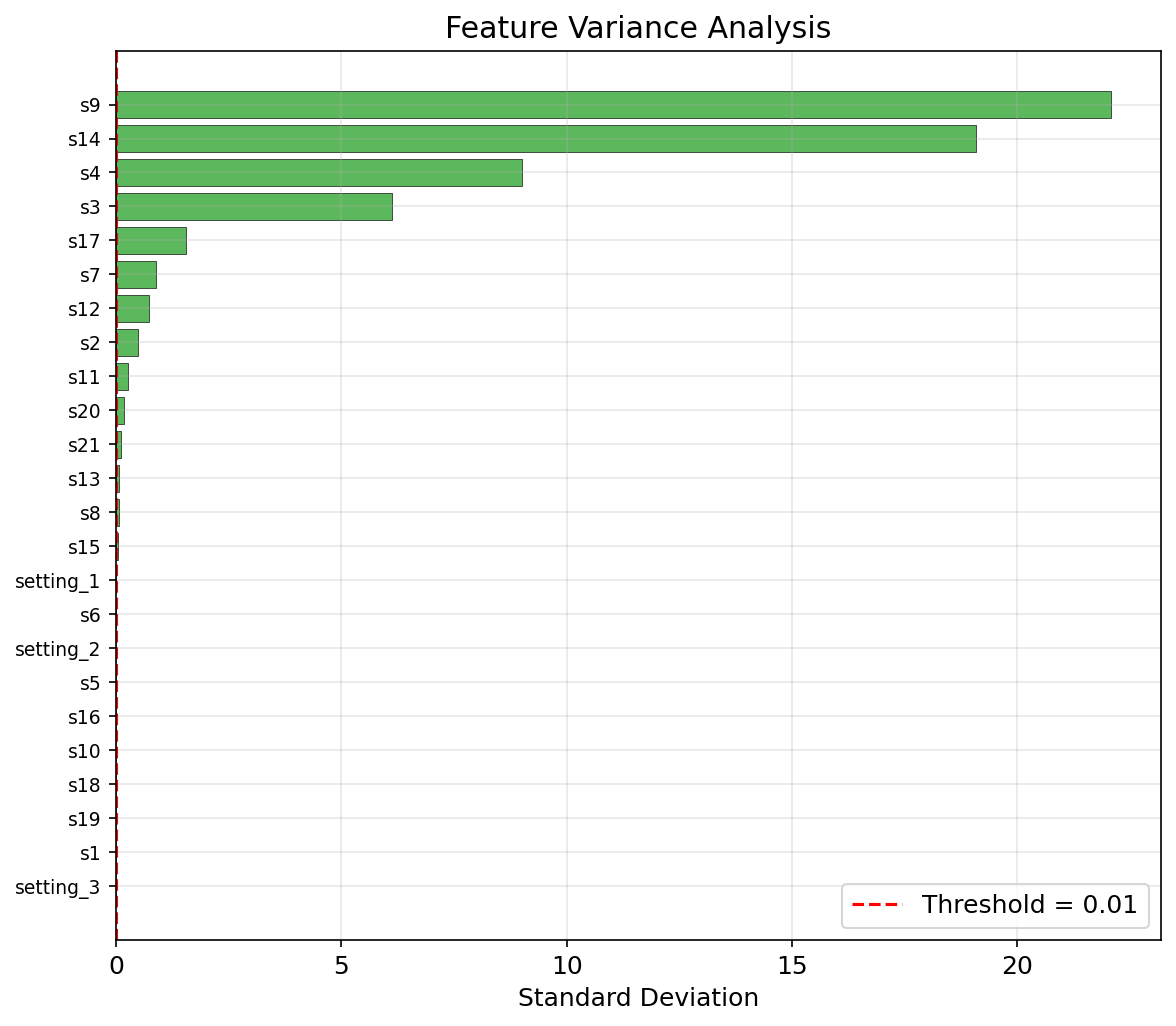
\includegraphics[width=\textwidth]{eda_variance.png}
    \caption{Feature variance (std). Red: removed.}
    \label{fig:eda_var}
\end{subfigure}
\hfill
\begin{subfigure}[t]{0.48\textwidth}
    \centering
    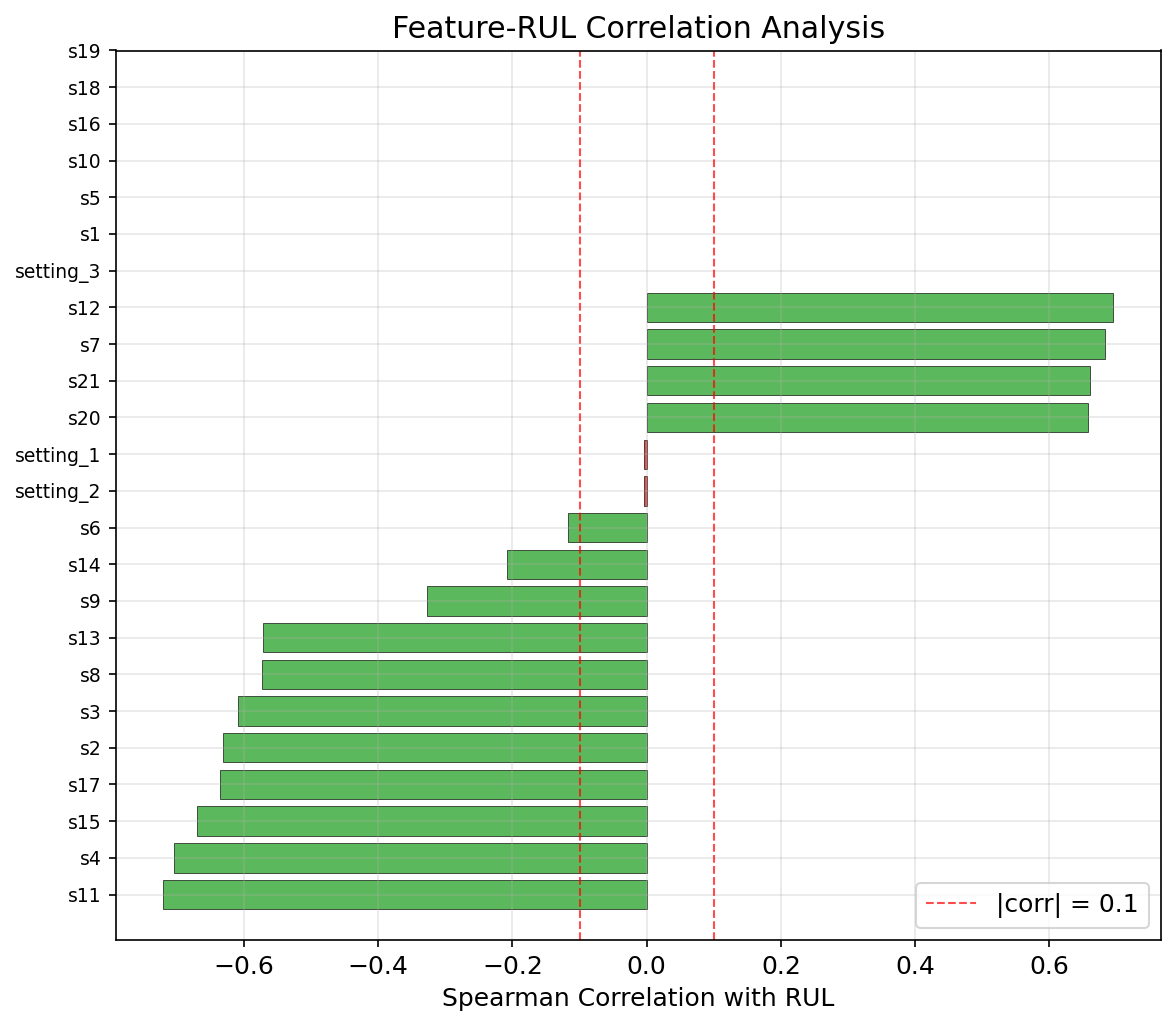
\includegraphics[width=\textwidth]{eda_correlation_rul.png}
    \caption{Spearman correlation with RUL.}
    \label{fig:eda_corr}
\end{subfigure}
\caption{Data-driven feature selection. (a)~10 near-constant features removed. (b)~All 14 retained features have $|\rho|{>}0.1$ with RUL.}
\label{fig:eda}
\end{figure}

\paragraph{Training.}
Adam optimiser ($\text{lr}{=}10^{-3}$, weight decay $10^{-4}$), batch size 32, gradient clipping ($\lVert\nabla\rVert \leq 1.0$).
ReduceLROnPlateau (factor 0.5, patience 5) and early stopping (patience 20).
Seed 42, CPU-only.

\paragraph{Metrics.}
\emph{Point prediction}: RMSE, MAE, $R^2$, NASA Score ($S = \sum_i e^{d_i/a}{-}1$, asymmetric with $a{=}13$/$10$).
\emph{Uncertainty quality}: PICP (95\% CI coverage), MPIW (interval width), NLL, calibration curve, and sparsification.

% ============================================================
\section{Results}
\label{sec:results}

\subsection{Point Prediction and Uncertainty Metrics}

Tables~\ref{tab:point} and \ref{tab:uq} summarise all quantitative results.
The probabilistic LSTM matches or outperforms the deterministic baseline on every point metric, confirming that the probabilistic formulation does not sacrifice accuracy.
The 17\% NASA Score reduction (351 vs.\ 424) is notable: the NLL objective produces more conservative predictions, reducing dangerous late estimates that incur heavy asymmetric penalties.

The 95\% prediction interval achieves 93\% coverage---slightly below nominal, indicating mild overconfidence---with a mean width of 51.64 cycles.
Uncertainty decomposition shows aleatoric variance accounts for ${\sim}$88\% of total variance (std 12.33 vs.\ epistemic 4.38).
This implies that data noise, not model capacity, is the dominant source of predictive uncertainty.

\begin{table}[t]
\caption{Point prediction metrics on C-MAPSS FD001 test set.}\label{tab:point}
\centering
\begin{tabular}{lcccc}
\toprule
Model & RMSE $\downarrow$ & MAE $\downarrow$ & $R^2$ $\uparrow$ & NASA Score $\downarrow$ \\
\midrule
Deterministic LSTM & 14.96 & 11.12 & 0.870 & 424.06 \\
\textbf{Probabilistic LSTM} & \textbf{14.84} & \textbf{11.08} & \textbf{0.872} & \textbf{351.07} \\
\bottomrule
\end{tabular}
\end{table}

\begin{table}[t]
\caption{Uncertainty quality metrics for the probabilistic LSTM.}\label{tab:uq}
\centering
\begin{tabular}{lcclc}
\toprule
Metric & Value & & Metric & Value \\
\midrule
PICP (95\% CI) & 0.93 & & Mean Aleatoric Std & 12.33 \\
MPIW (95\% CI) & 51.64 & & Mean Epistemic Std & 4.38 \\
NLL & 3.02 & & Mean Total Std & 13.17 \\
\bottomrule
\end{tabular}
\end{table}

\subsection{Qualitative Analysis}

\begin{figure}[!t]
\centering
\begin{subfigure}[t]{0.48\textwidth}
    \centering
    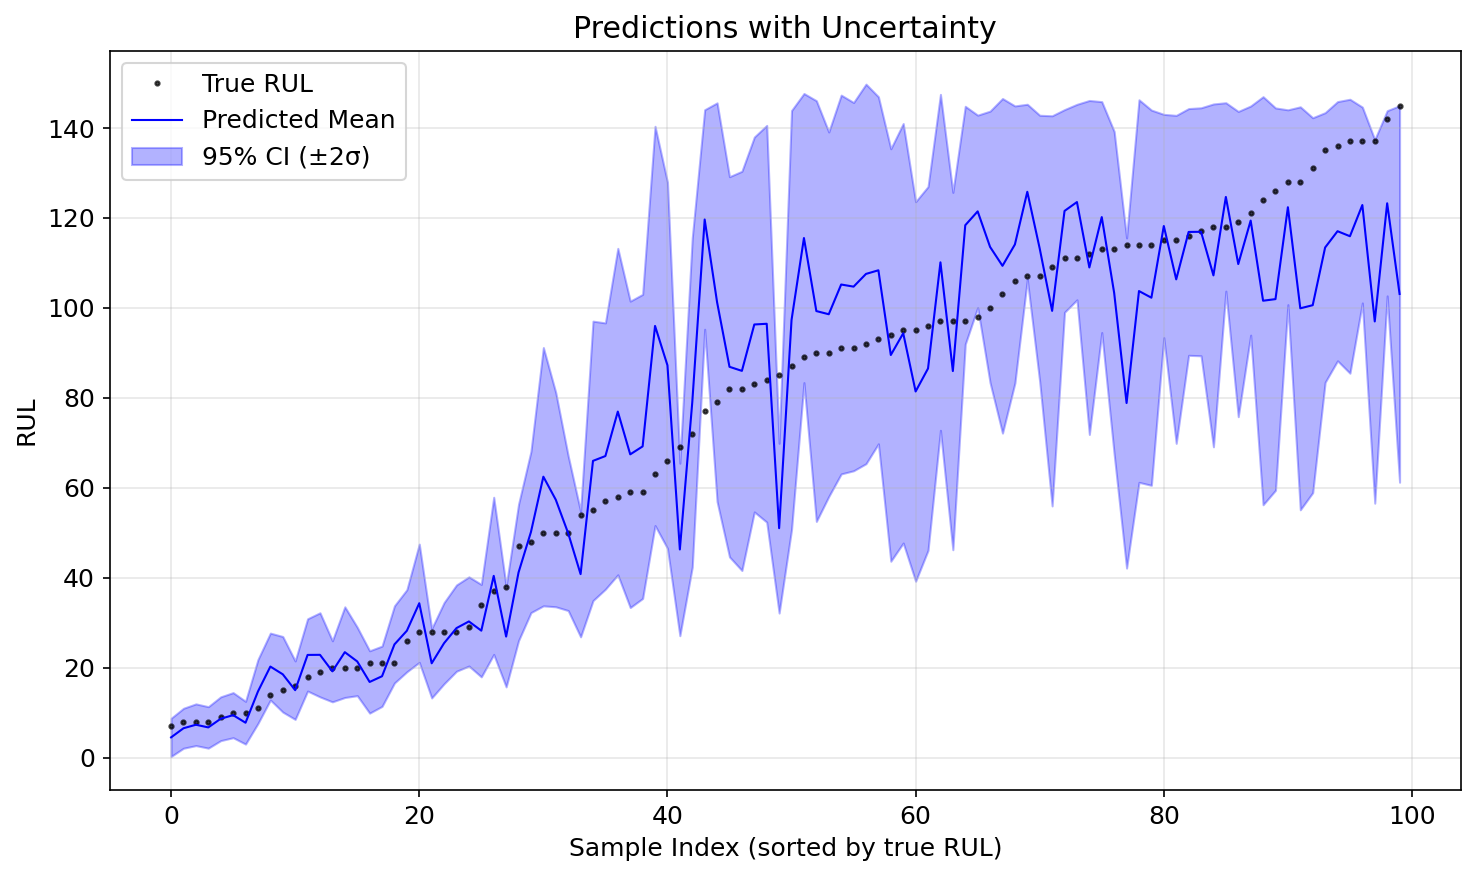
\includegraphics[width=\textwidth]{predictions_uncertainty.png}
    \caption{Predictions with 95\% CI ($\pm 2\sigma_{\text{total}}$).}
    \label{fig:pred_unc}
\end{subfigure}
\hfill
\begin{subfigure}[t]{0.48\textwidth}
    \centering
    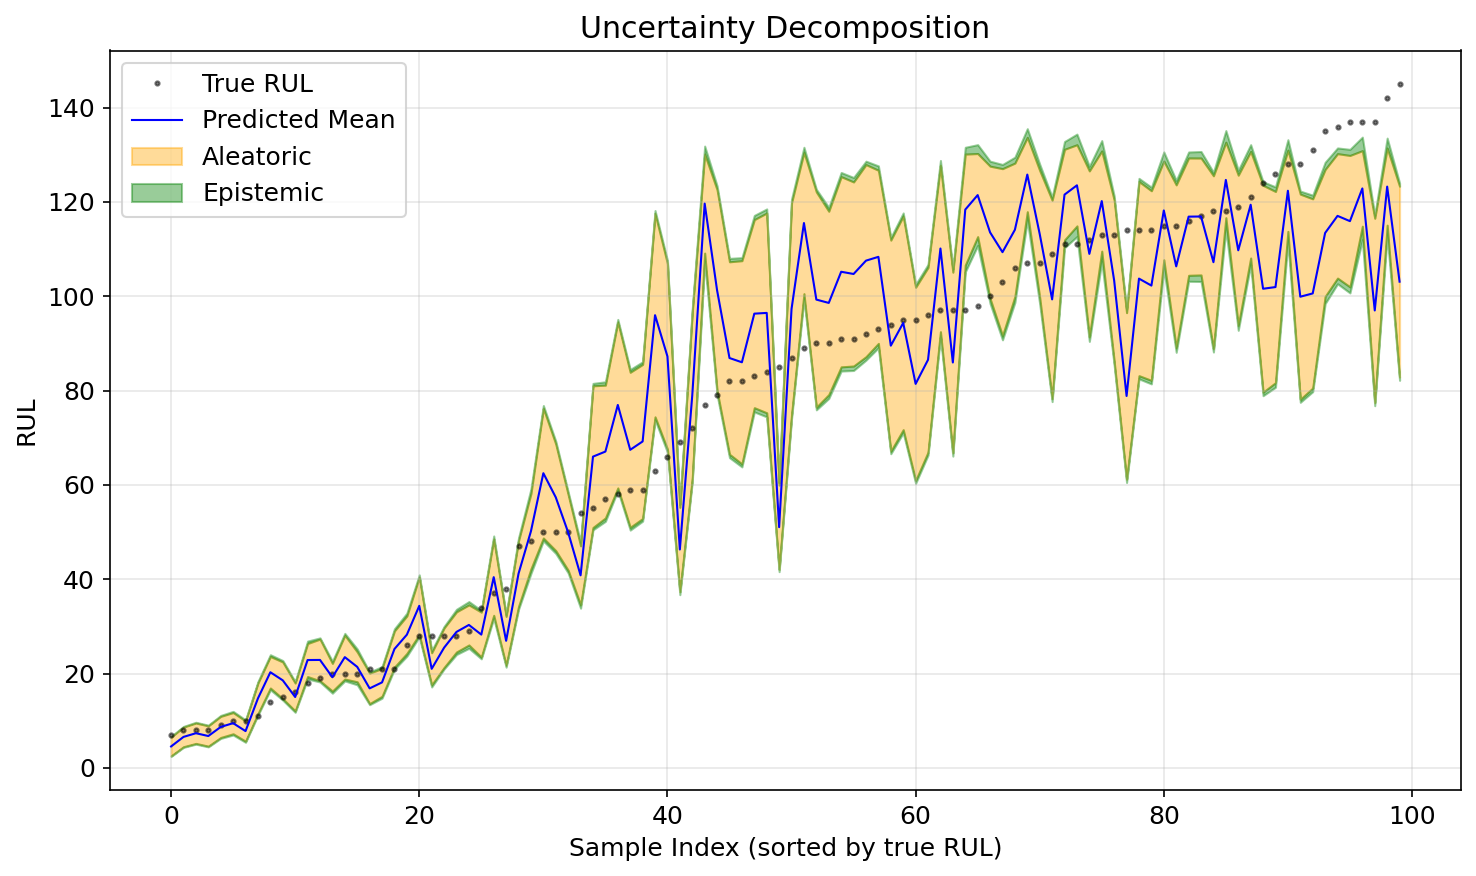
\includegraphics[width=\textwidth]{uncertainty_decomposition.png}
    \caption{Aleatoric (orange) vs.\ epistemic (green).}
    \label{fig:decomp}
\end{subfigure}\\[4pt]
\begin{subfigure}[t]{0.48\textwidth}
    \centering
    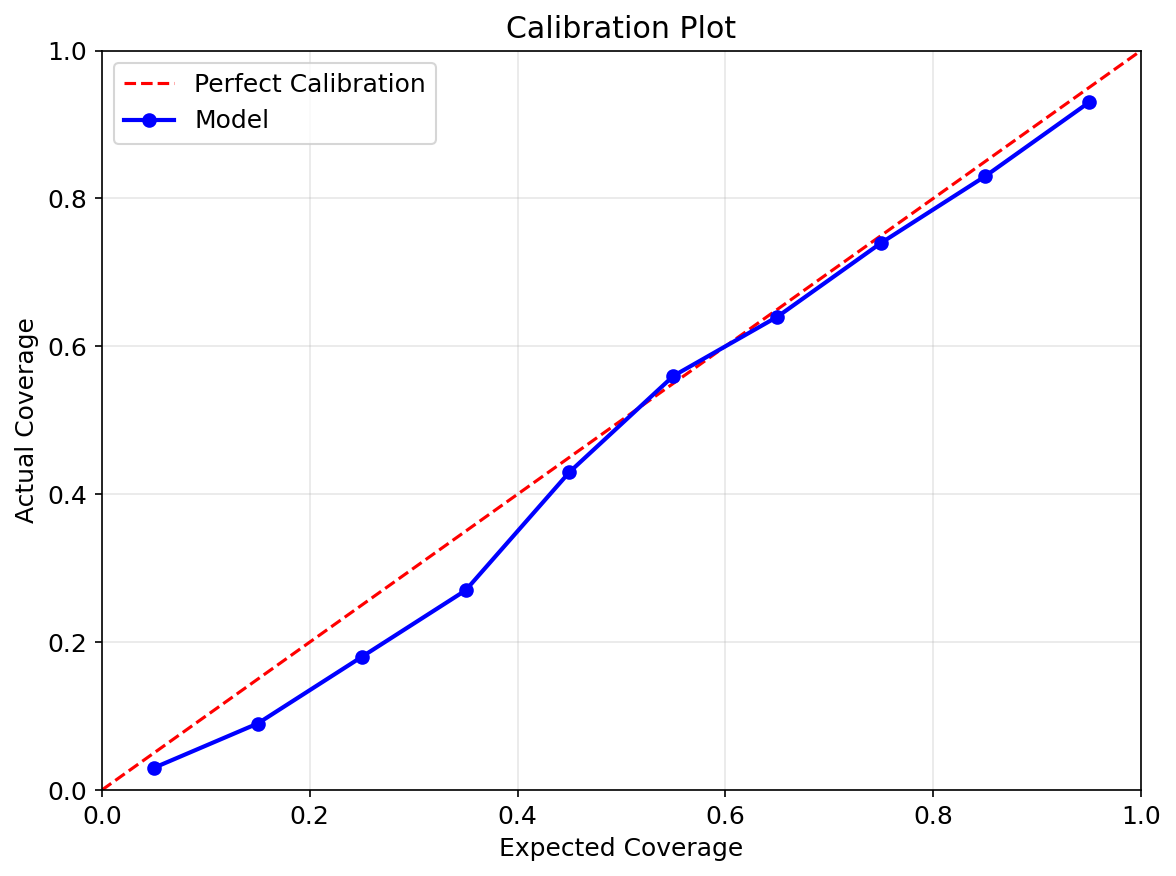
\includegraphics[width=\textwidth]{calibration.png}
    \caption{Calibration: actual vs.\ expected coverage.}
    \label{fig:calib}
\end{subfigure}
\hfill
\begin{subfigure}[t]{0.48\textwidth}
    \centering
    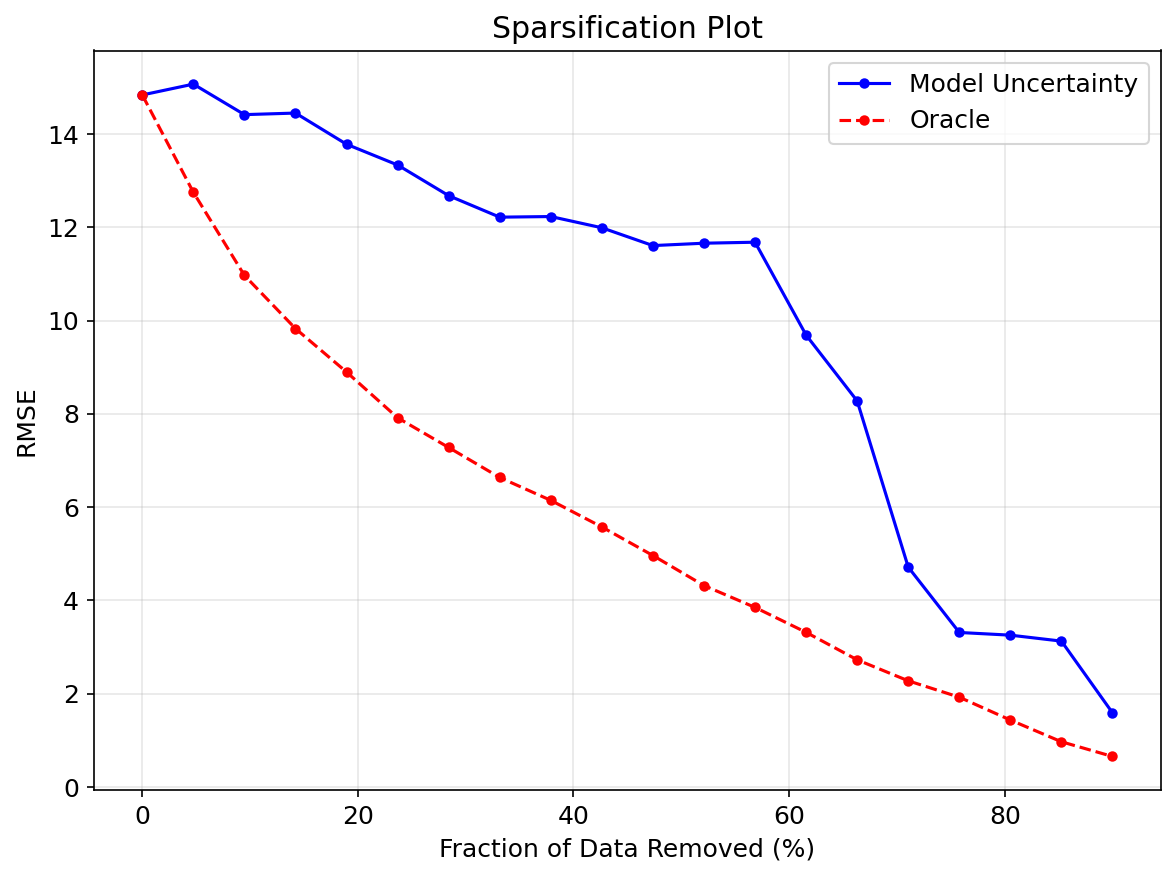
\includegraphics[width=\textwidth]{sparsification.png}
    \caption{Sparsification: RMSE vs.\ fraction removed.}
    \label{fig:sparse}
\end{subfigure}
\caption{Uncertainty analysis. (a)~Confidence bands narrow at low RUL, widen at high RUL. (b)~Aleatoric uncertainty dominates. (c)~Calibration tracks the diagonal. (d)~Removing high-uncertainty samples reduces RMSE, tracking the oracle.}
\label{fig:unc_results}
\end{figure}

Fig.~\ref{fig:unc_results}a shows 95\% confidence bands that narrow for advanced-degradation engines.
Fig.~\ref{fig:unc_results}b confirms aleatoric uncertainty dominates, indicating sufficient model capacity.
The calibration curve (Fig.~\ref{fig:unc_results}c) tracks the diagonal, and the sparsification plot (Fig.~\ref{fig:unc_results}d) confirms the model identifies \emph{which} predictions are unreliable---a prerequisite for risk-aware deployment.

% ============================================================
\section{Discussion}
\label{sec:discussion}

\paragraph{NLL as implicit regulariser.}
The 17\% NASA Score improvement (351 vs.\ 424, Table~\ref{tab:point}) suggests NLL implicitly regularises predictions, discouraging overconfident high-RUL estimates that incur heavy asymmetric penalties.

\paragraph{Aleatoric dominance.}
The 88/12 variance ratio (Table~\ref{tab:uq}) indicates sufficient model capacity for FD001; data quality improvements would reduce uncertainty more effectively than architectural changes.

\paragraph{Limitations and future work.}
The 93\% PICP reflects mild overconfidence from the Gaussian assumption; alternative distributions could help.
MC Dropout ($T{=}100$) increases inference cost; evidential deep learning~\cite{amini2020deep} warrants investigation.
Future work includes Transformer encoders for interpretable uncertainty, multi-condition evaluation on FD002--FD004, and cost-sensitive maintenance scheduling.

% ============================================================
\begin{credits}
\subsubsection{\discintname}
The authors have no competing interests to declare.
\end{credits}

\begin{thebibliography}{15}

\bibitem{lei2018machinery}
Lei, Y., Li, N., Guo, L., Li, N., Yan, T., Lin, J.:
Machinery health prognostics: A systematic review from data acquisition to RUL prediction.
Mech.\ Syst.\ Signal Process.\ \textbf{104}, 799--834 (2018)

\bibitem{sateesh2016deep}
Sateesh Babu, G., Zhao, P., Li, X.-L.:
Deep convolutional neural network based regression approach for estimation of remaining useful life.
In: DASFAA, LNCS, vol.~9642, pp.~214--228. Springer (2016)

\bibitem{li2018remaining}
Li, X., Ding, Q., Sun, J.-Q.:
Remaining useful life estimation in prognostics using deep convolution neural networks.
Reliab.\ Eng.\ Syst.\ Saf.\ \textbf{172}, 1--11 (2018)

\bibitem{zheng2017long}
Zheng, S., Ristovski, K., Farahat, A., Gupta, C.:
Long short-term memory network for remaining useful life estimation.
In: IEEE ICPHM, pp.~88--95 (2017)

\bibitem{wu2018remaining}
Wu, Y., Yuan, M., Dong, S., Lin, L., Liu, Y.:
Remaining useful life estimation of engineered systems using vanilla LSTM neural networks.
Neurocomputing \textbf{275}, 167--179 (2018)

\bibitem{mo2021multi}
Mo, Y., Wu, Q., Li, X., Huang, B.:
Remaining useful life estimation via transformer encoder enhanced by a gated convolutional unit.
J.\ Intell.\ Manuf.\ \textbf{32}, 1997--2006 (2021)

\bibitem{kiureghian2009aleatory}
Der Kiureghian, A., Ditlevsen, O.:
Aleatory or epistemic? Does it matter?
Struct.\ Saf.\ \textbf{31}(2), 105--112 (2009)

\bibitem{blundell2015weight}
Blundell, C., Cornebise, J., Kavukcuoglu, K., Wierstra, D.:
Weight uncertainty in neural networks.
In: ICML, pp.~1613--1622 (2015)

\bibitem{lakshminarayanan2017simple}
Lakshminarayanan, B., Pritzel, A., Blundell, C.:
Simple and scalable predictive uncertainty estimation using deep ensembles.
In: NeurIPS, vol.~30 (2017)

\bibitem{gal2016dropout}
Gal, Y., Ghahramani, Z.:
Dropout as a Bayesian approximation: Representing model uncertainty in deep learning.
In: ICML, pp.~1050--1059 (2016)

\bibitem{nix1994estimating}
Nix, D.A., Weigend, A.S.:
Estimating the mean and variance of the target probability distribution.
In: IEEE ICNN, vol.~1, pp.~55--60 (1994)

\bibitem{kraus2019forecasting}
Kraus, M., Feuerriegel, S.:
Forecasting remaining useful life: Interpretable deep learning approach via variational Bayesian inferences.
Decis.\ Support Syst.\ \textbf{125}, 113100 (2019)

\bibitem{biggio2021prognostics}
Biggio, L., Wiber, A., Kastanis, I., Alberti, C., Schaer, M.:
Prognostics and health management of industrial assets: Current progress and road ahead.
Front.\ Artif.\ Intell.\ \textbf{3}, 578613 (2021)

\bibitem{heimes2008recurrent}
Heimes, F.O.:
Recurrent neural networks for remaining useful life estimation.
In: IEEE ICPHM, pp.~1--6 (2008)

\bibitem{saxena2008damage}
Saxena, A., Goebel, K., Simon, D., Eklund, N.:
Damage propagation modeling for aircraft engine run-to-failure simulation.
In: IEEE ICPHM, pp.~1--9 (2008)

\bibitem{amini2020deep}
Amini, A., Schwarting, W., Soleimany, A., Rus, D.:
Deep evidential regression.
In: NeurIPS, vol.~33, pp.~14927--14937 (2020)

\end{thebibliography}

\end{document}
